%
% $Id: chapter2.tex 2612 2008-06-03 18:32:54Z jozinke $
%

\chapter{Background}
\label{sec:background}

The following section introduces the concept of \ac{HIDS} with the specific example of Fail2ban and presents the problem setting 
this thesis aims to solve. In addition to that, an overview over common types of Inter-Process Communication and existing IPC based logging solution is given. 
Finally, external libraries and other software used for the implementation and evaluation of the proof of concept IPS are introduced.    

\section{Host-based Intrusion Detection / Prevention}
\label{sec:hids}
Intrusion Detection Systems are tasked with monitoring and collecting data from target systems, which is then further processed and analyzed, to identify 
potential threads and facilitate a response \cite{vigna2006}.
The idea of specialized software for detecting intrusion attempts and other 
security threads goes as far back as 1980, when James Anderson published a study on 
``Computer security threat monitoring and surveillance'', suggesting the use of automated tools to assist with security monitoring\cite{anderson1980}. In 1987, Dorothy
Denning presented a seminal model for Intrusion Detection Systems\ac{IDS}, that proposed the use of pattern matching based on
statistical analysis of audit records generated by a system, in order to detect abnormal user behavior \cite{denning1987}. 
Intrusion Detection Systems in general, can collect data from a multitude of sources. This allows for the distinction between network-based intrusion detection systems \ac{NIDS} and host-based introduction detection systems \ac{HIDS}. \ac{NIDS}
monitor network interfaces and analyze captured traffic, while \ac{HIDS} gather information directly provided by the hosts under their supervision. For the latter, this includes event logs of applications, as well as operating system \ac{OS} based information,
such as user logins, file system operations or systemcalls. For analysis of the accumulated data, there a two commonly deployed strategies: 1. Misuse based detection relies on predefined 
patterns of misuse or malicious behavior, which are then matched against the observed data. 2. Anomaly based detection uses statistical analysis to identify significant deviations
from normally observed behavior, which, in principal, enables the detection of attack patterns, that have not been previously observed \cite{vigna2006}. 

\subsection{Fail2ban}
\label{sec:fail2ban}

Fail2ban is a open source Intrusion Prevention System \ac{IPS}, that is widely used to protect hosts against a range of network-based attacks, such as, for instance, brute-force login attempts\cite{fail2ban}. Intrusion prevention system constitute
a special class of \ac{IDS}, that not only detects an intrusion attempt, but also initiates an active response, with the aim of preventing or mitigating the attack. To identify potentially malicious clients,
Fail2ban uses a misuse detection approach based on application logs. For configured applications, Fail2ban actively monitors their log and parses new entries based on a predefined filter. Fail2ban uses configuration units called `jails'  
, that allow for the customization to different applications. A jail defines a path to a application log, the filter being applied to the log messages within the logfile and an action, that
is executed on client matching the filter criteria. In addition to that, jails contain further parameters, such as the threshold of matches a client need to reach, in order for the action to be executed,
as well as the duration of that action. The filter component of a jail defines a set of regular expressions \ac{REGEX}, that are used to identify certain events in a log, for example an unsuccessful login attempts or the 
exceeding of a request rate limit. The filter also obtains a clients IP address, as well as the date and time of the log messages, to determine, if the event occurred within a relevant time frame. 
Most commonly, the action issued by Fail2ban for eligible clients, is to ban the clients IP address for the duration configured in the associated jail. Fail2ban facilitates this via an iptables entry. 
Iptables is a utility program for Linux systems, that allows the interaction with the netfilter Kernel framework to implement packet filtering rules. When banning a client, Fail2ban add a iptables rule for the clients IP address that leads 
to the dropping of all subsequent network packets from that address, for as long as the rule is active.
\par
Fail2bans netfilter based approach of packet filtering has disadvantage of scaling poorly for large traffic rates, since packets need to traverse several processing steps of the kernel network stack before they are ultimately discarded.
In his master thesis, Florian Mikolajczak therefore proposed the usage of eBPF programs, as a more efficient way of implementing packet filtering for intrusion prevention systems\cite{mikolajczak2022}. The extended Berkley Packet Filter \ac{eBPF}      
is an interface of the Linux kernel, that allows the event based execution of verified user defined programs within the kernel. Packet filtering through \ac{eBPF} can be facilitated with an \ac{eBPF} program,
that is executed on incoming packets and delivers a verdict, of wether the packets should be dropped or further processed by the Kernel. Via the Express Datapath \ac{XDP}, \ac{eBPF} programs can be attached to different hooks in 
the packet processing pipeline. For supported devices, programs can be attached in XPD\_DRIVER mode, where they are executed as part of the network device diver routine, very early into the packet processing. Florian Mikolajczak adapted an existing \ac{eBPF} program by (name \cite{}) to handle
IP version 6 \ac{IPv6} as well and integrated it with Fail2ban to replace netfilter-based packet filtering. While he was able to demonstrate significant performance improvements over netfilter-based filtering, his measurents 
revealed, that Fail2ban has significant performance issues, when faced with a large influx of log messages. 

\begin{figure}[h!]
	\label{fig:fail2ban:mikolajczak2022}
	\centering
	\scriptsize
    \centerline{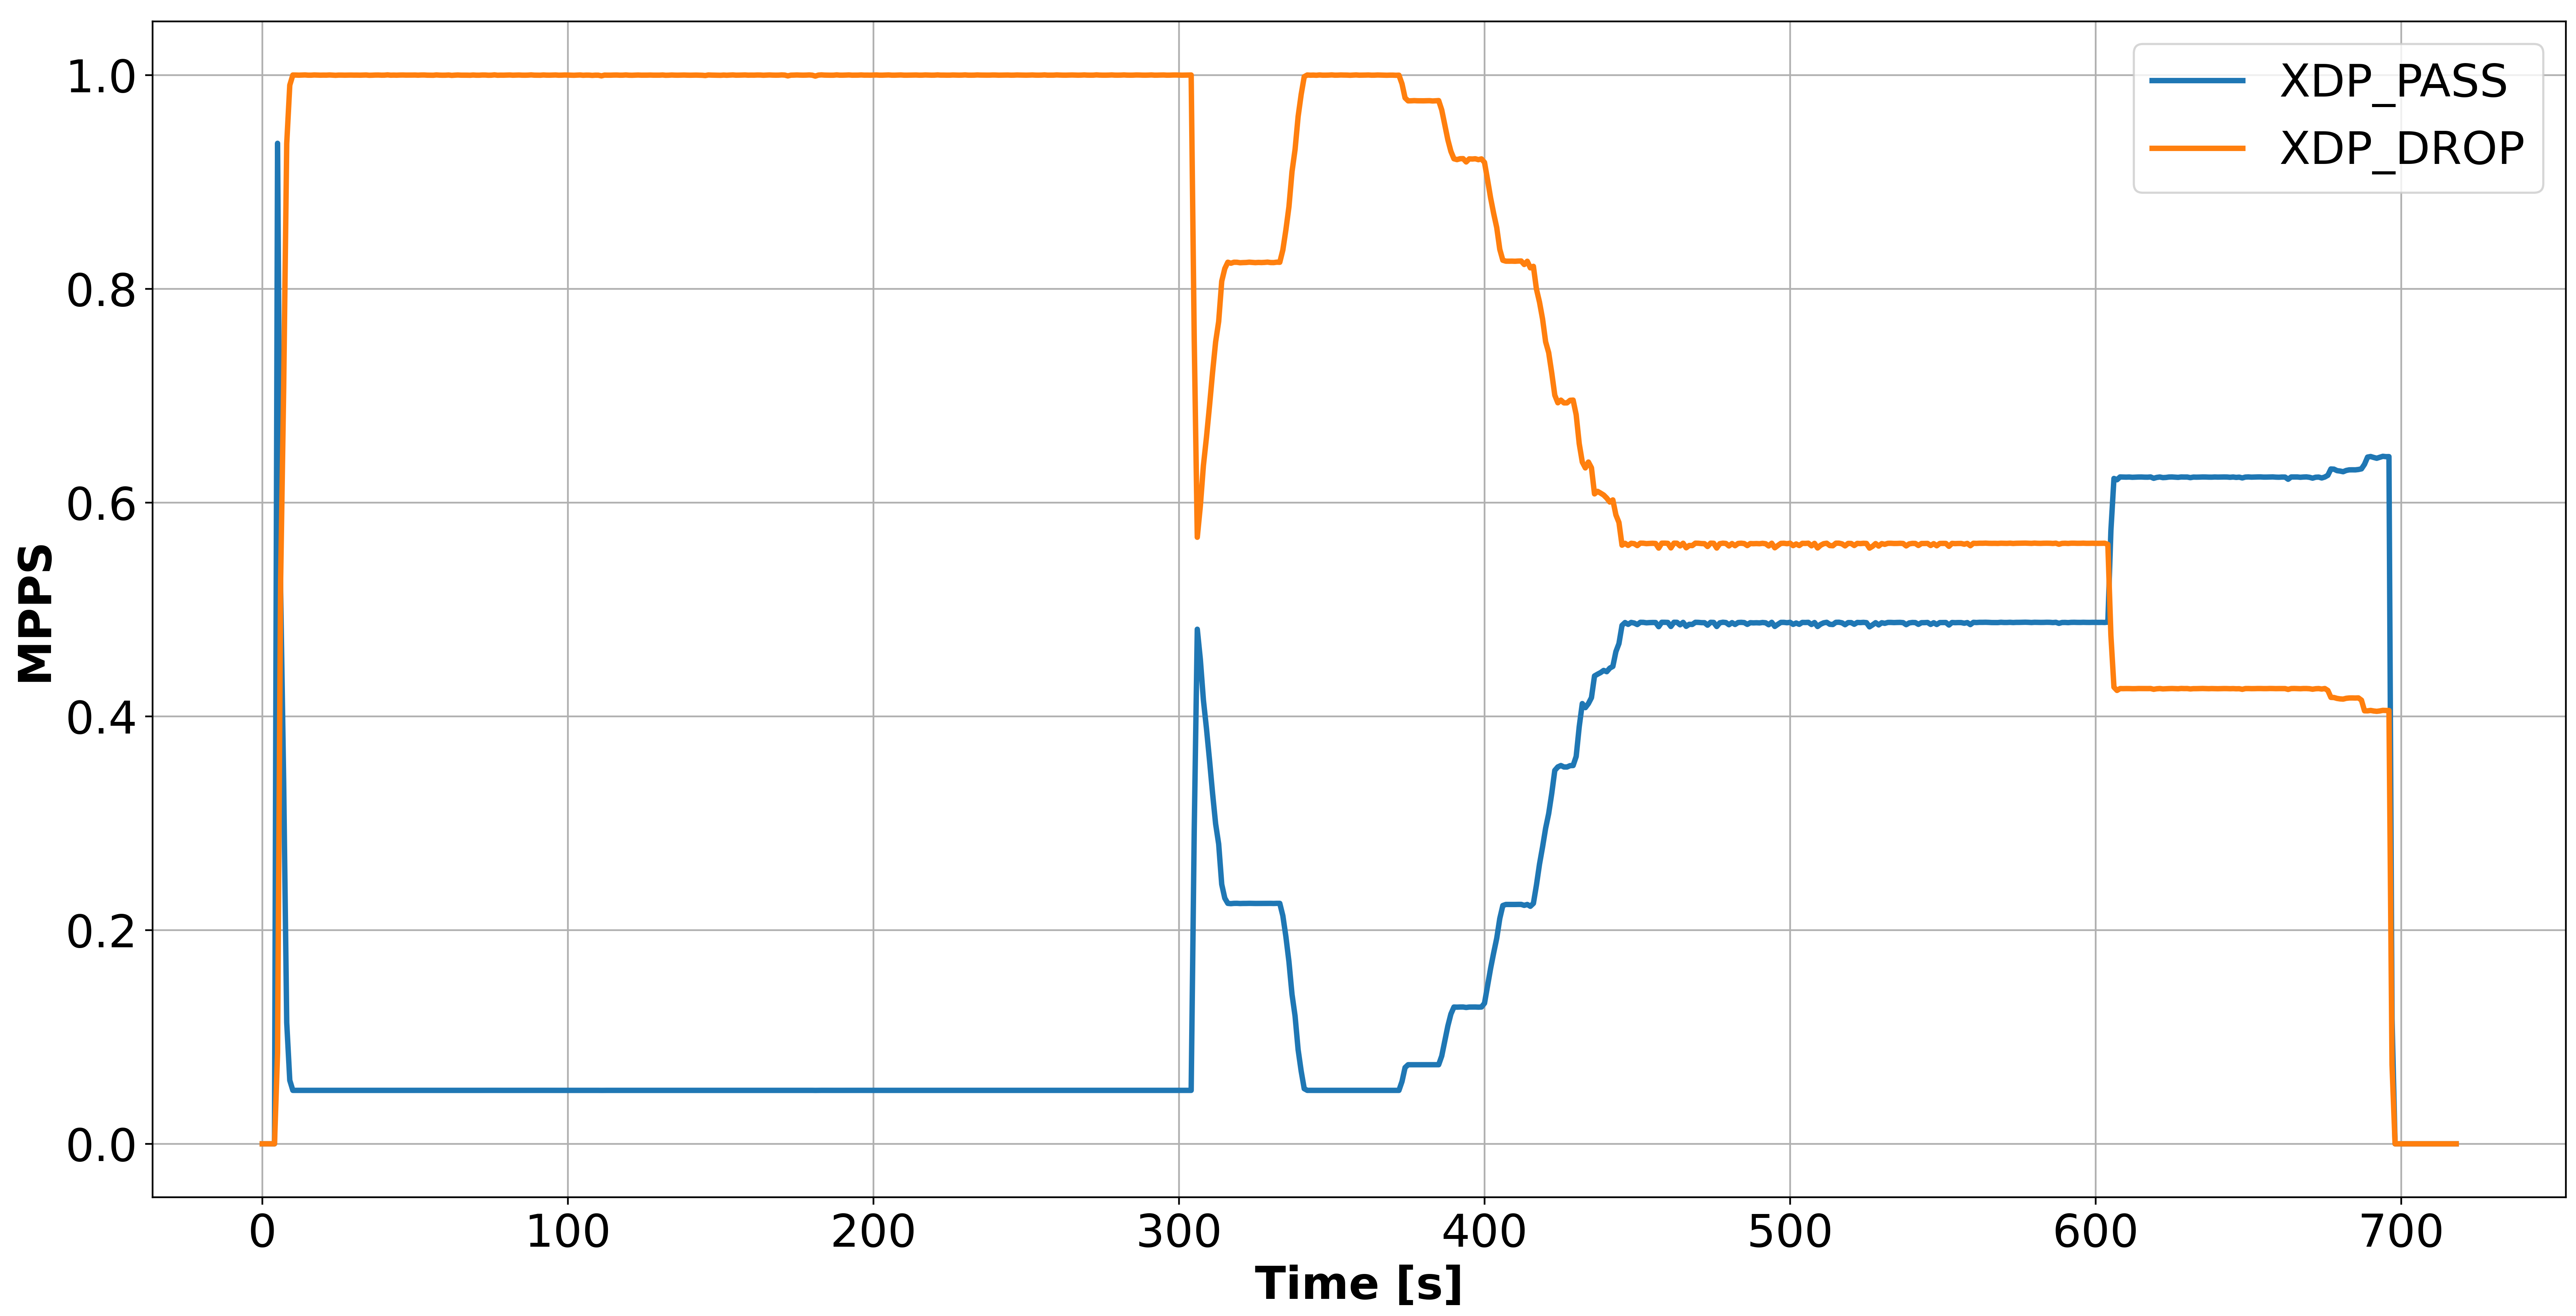
\includegraphics[width=1.2\textwidth]{images/Fail2Ban2.png}}
    \caption[Fail2ban measurement by \cite{mikolajczak2022}]{Results of experiment 1 from the  master thesis of Florian Mikolajczak\cite{mikolajczak2022}. Fail2Ban, even in conjunction with more efficient \ac{eBPF} filtering, performs poorly for large traffic rates.}
\end{figure}

Figure \ref{fig:fail2ban:mikolajczak2022} shows the results of the Fail2ban measurement conducted by Florian Mikolajczak. In the experiment, a BIND9 DNS Server received unwanted requests at a rate of 1 million packets per second \ac{PPS} from 254 different clients,
which resulted in corresponding entries in the rate-limit log. Fail2ban was configured to ban clients with rate limit violations for 300 seconds. Initially, the performance was as expected. However, after 
the end of the first ban cycle, Fail2ban failed to renew the ban for some clients, leading to a significant amount of unwanted traffic still reaching the application. Closer inspection of Fail2bans behavior indicated,
that the performance issues are a result of slow logfile parsing. Fail2bans rate of processing log entries appeared to be exceeded by rate of new entries, leading to Fail2ban falling increasingly further behind
in the processing of logged events. This constitutes a problem, as it essentially makes Fail2ban and by extension the protected host, vulnerable to \ac{DOS} attacks. The primary goal of this thesis, will therefore be the development 
of an \ac{IPC}-based logging architecture, that is able to handle the scenario above.          


\section{Inter-Process Communication}
\label{sec:ipc}

\subsection{Types of IPC}
\label{sec:ipc_types}

Inter-process communication allows the exchange of data between different processes through APIs provided by the operating system. Since the
the development environment for this thesis will be Linux, I will focus on \ac{IPC} APIs that are available on UNIX-like systems.
A commonly used mechanism for sharing large amount of data between two processes on the same system is shared memory \cite[p.301ff.]{stevens1998ipc}.
Shared memory allows the allocation of memory segment in RAM, that can mapped into address space of several processes. The memory segment has associated file associated permissions, that 
allow the creating process to control read and write access by other processes. Linux provides two main ways of creating
shared memory in the System V shared memory API \cite{systemvshm} and the newer POSIX shared memory API \cite{posixshm}. Processes can essentially treat shared memory like 
any other valid memory in their address space, which allows for flexible application. A disadvantage of shared memory, at least for the aforementioned APIs, is its restriction 
to the local system boundaries, though solutions for network based remote direct memory access (RDMA) exist\cite{recio2007}.
\par 
Pipes, specifically named pipes, are a way of facilitating unidirectional data transfer between processes on a UNIX system. Named pipes have a read and a write end and are  
associated with a special file in the filesystem, which can be accessed by different processes. Pipe can be written to and read from via the write and read system calls. The data is transmitted in 
a first-in first-out (FIFO) manner, hence why named pipes are also referred to as FIFOs. The maximum capacity up to which a pipe can buffer data is limited, which by default is 65535 bytes on linux. \cite{pipe}   
\par
Sockets are another common\ac{ICP} type for data transfer, that allow for one-to-one as well as one-to-many 
communication via a range of protocols\cite[p.57ff.]{stevens1998sock}. Sockets send data in formatted packets, that can be transmitted on a local host or via a network. For communication on a local system, UNIX systems offer UNIX Domain sockets. UNIX Domain sockets can be bound to a valid path in the filesystem, which serves the way of addressing
the socket from another processes \cite{unixsock}. For data transfer beyond the local system, the Internet protocol \ac{IP} in conjunction with the Transmission Control Protocol \ac{TCP} or User Datagram 
Protocol \ac{UDP} is most common. TCP offers connection oriented data transmission, that requires an orderly connection establishment through a handshake between the commutating parties. It further ensures a reliable transfer of data, by       
detecting transmission errors trough acknowledgment and retransmitting unacknowledged packets. \ac{UDP} in contrast, provides no guarantees on reliable transfer, with the benefit of lower latency and less communication overhead. \cite[p.29ff.]{stevens1998sock}
\par
Finally, message queues are another commonly used \ac{IPC} mechanism that allow the exchange of messages between processes. Linux natively supports the System V \cite{systemvshm} and POSIX \cite{posixmsq} message queue APIs, but third party
implementations exist as well, for instance the ZeroMQ message queue library \cite{zeromq}. Message queues essentially function as a buffer, which can store messages up to a certain capacity. A writing process adds messages to the queue, while
reading processes remove messages from the queue. Unlike with sockets, writing and reading can occur asynchronously i.e. messages do not have to be read immediately after being added to a queue. ZeroMQ specifically supports a range of communication 
patterns, among them the publish-subscribe pattern, where a writer sends messages to multiple subscribed readers or the request-reply pattern, that can be used to implement remote procedure calls.         

\subsection{IPC based logging}
\label{sec:ipc_logging}
Other than traditional logfiles, 

Syslog, Rsyslog

\section{Special Software}
\label{sec:softwar}

\subsection{Hyperscan}
\label{sec:hyperscan}

Hyperscan is a open source regular expressions matching engine developed by Intel. 
It is specifically designed for high performance use cases, such as the application in security contexts and is being used by the intrusion detection systems Snort and Suricata \cite{hyperscan}.  
The process of regular expressions matching with Hyperscan is separated into compile- and run-time. At compile-time a set regular expressions in string representation are compiled into a 
database, with additional configuration options  

\subsection{io\_uring}
\label{sec:io_uring}

\subsection{Trex}
\label{sec:trex}
